\chapter{Weighted Interval Scheduling
  Problem}

Abbiamo visto che un algoritmo \textbf{greedy} produce una soluzione
ottimale per l'Interval Scheduling Problem, in cui l'obiettivo è
accettare un insieme di intervalli non sovrapposti il più ampio
possibile. \textbf{Il Weighted Interval Scheduling Problem} è una
versione più \textbf{generale}, in cui ogni intervallo ha un certo
valore (o peso), e vogliamo accettare un insieme di valore massimo.
\\
\\
Questo problema ha l'obiettivo di ottenere un insieme (il più grande
possibile) di intervalli non sovrapposti (overlapping). Per la versione
non pesata (Interval Scheduling Problem in cui weight=1) esiste uno
specifico algoritmo \textbf{Greedy} che è in grado di trovare la
soluzione ottima, tuttavia nella versione più generale, ovvero la
versione pesata (\textbf{il Weighted Interval Scheduling Problem},
weight $\neq$ 1), è necessario utilizzare la programmazione dinamica.
\\
\\


\begin{figure}[H]
      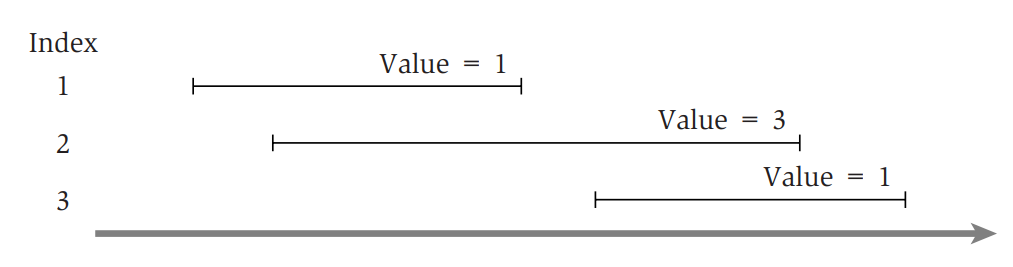
\includegraphics[width=\textwidth]{capitoli/programmazione_dinamica/imgs/weigted_interval_scheduling.png}
      \centering
      \caption{Un esempio di weighted interval scheduling}
      %\label{fig:wis}
\end{figure}


\section{Descrizione del problema}

\begin{itemize}
      \item
            $n$: un intero che rappresenta l'indice dell'intervallo (job)
      \item
            $s_i$: tempo di inizio dell'intervallo $i$
      \item
            $f_i$: tempo di fine dell'intervallo $i$
      \item
            $v_i$: peso dell'intervallo $i$
      \item
            Due job sono \textbf{compatibili} se non si sovrappongono.
      \item
            $p(j)$: ritorna l'indice più grande $i$, con $i < j$, del primo
            intervallo compatibile con l'intervallo $j$, considerando il fatto
            che gli intervalli sono ordinati in ordine non decrescente in base a
            $f_i$
      \item
            $\mathcal{O}_j$: rappresenta la soluzione ottima al problema
            calcolato sull'insieme $\{1, \ldots, j\}$
      \item
            $OPT(j)$: rappresenta il valore della soluzione ottima
            $\mathcal{O}_j$
\end{itemize}

\begin{figure}[H]
      \centering
      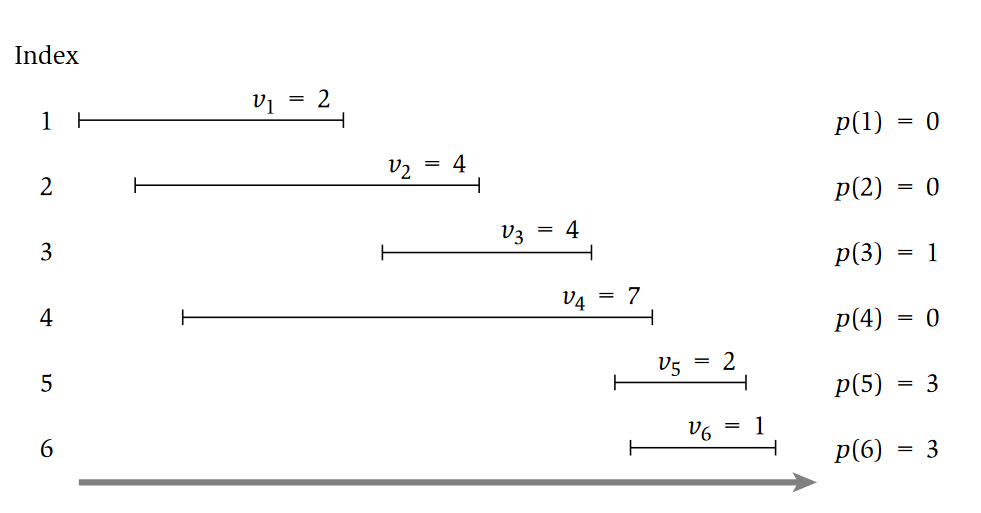
\includegraphics[width=15cm, keepaspectratio]{capitoli/programmazione_dinamica/imgs/wis_instance.png}
      \caption{Si può vedere come funziona effettivamente la funzione $p(i)$}
\end{figure}

\subsection{Goal:}

\begin{itemize}
      \item L'obiettivo del problema attuale è quello di trovare un sottoinsieme
            $S \subseteq \{1, \ldots, n\}$ di intervalli mutualmente compatibili
            che vanno a massimizzare la somma dei pesi degli intervalli
            selezionati $\sum_{i \in S} v_i$.
\end{itemize}


\section{Greedy Version; Earliest Finish Time First}

Considero i job in ordine non decrescente di $f_j$, aggiungo un job
alla soluzione se è compatibile con il precedente.\\
È corretto se i pesi sono tutti 1, ma \textbf{fallisce} clamorosamente
nella versione pesata.

\section{Dynamic Version}

Come prima cosa definiamo il metodo per calcolare $OPT(j)$. Il
problema è una \textbf{\emph{scelta binaria}} che va a decidere se il
job di indice $j$ verrà \textbf{incluso} nella soluzione
\textbf{oppure no}, basandosi sul valore ritornato dalla seguente
formula (si considerano sempre i job in ordine non decrescente rispetto
a $f_i$):

$$
      OPT(j) = max(v_j + OPT(p(j)), \ \ OPT(j-1))
$$

Questo può essere anche visto come una \textbf{disequazione}:

$$
      v_j + OPT(p(j)) \geq OPT(j-1)
$$

che \textbf{se vera}, includerà $j$ nella soluzione ottimale.


\section{Brute Force}

Scrivendo tutto sotto forma di algoritmo ricorsivo avremmo che:

\begin{lstlisting}[language=Python, mathescape=true]
  Input: n, s[1..n], f[1..n], v[1..n]
  Sort jobs by finish time so that f[1] $\le$ f[2] $\le$ ... $\le$ f[n]. 
  Compute p[1], p[2], ..., p[n].
  
  function Compute-Opt(j){
      if (j == 0)
          return 0
      else
          return max(vj+Compute-Opt(p(j)), Compute-Opt(j - 1))
  }
\end{lstlisting}

Costruendo l'albero della ricorsione dell'algoritmo si nota che la
complessità temporale è \textbf{esponenziale}. Questo perchè seguendo
questo approccio, venogno calcolati più volte gli stessi sottoproblemi,
i quali si espandono come un albero binario. Il numero di chiamate
ricorsive cresce come la \textbf{sequenza di fibonacci}.

\begin{figure}[H]
      \centering
      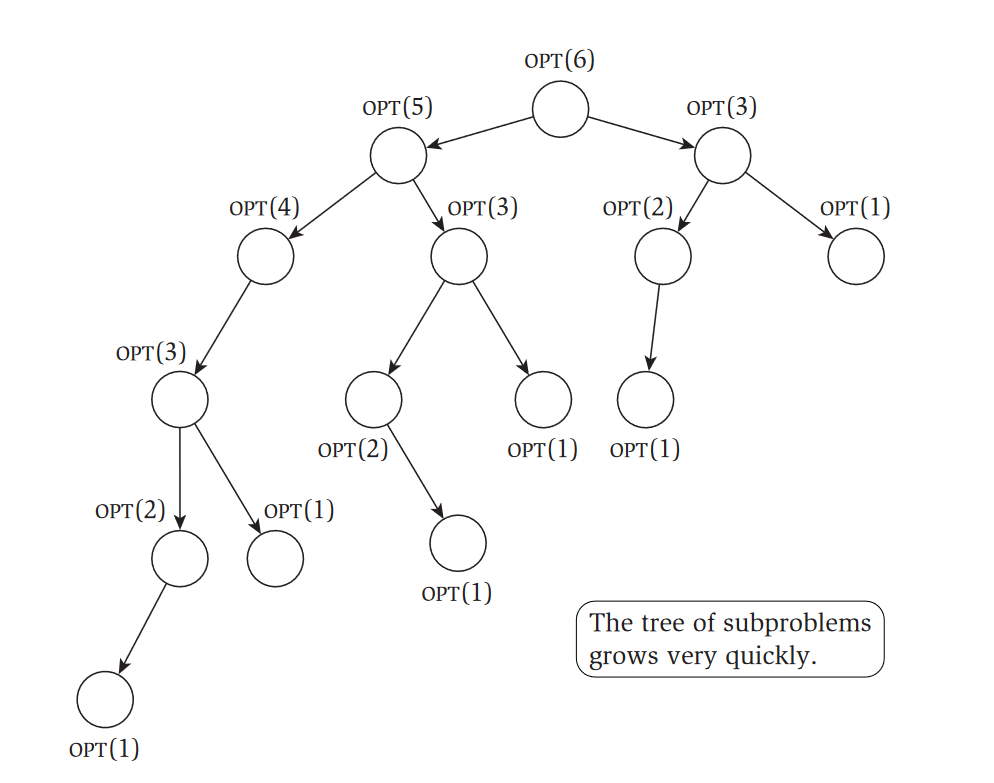
\includegraphics[width=10cm]{capitoli/programmazione_dinamica/imgs/wis_subproblem_tree.png}
      \caption{L'albero dei sottoproblemi chiamati da \texttt{Compute-Opt}}
\end{figure}

Una soluzione è quella di utilizzare la tecnica della
\textbf{Memoization} che evita di ricalcolare $OPT$ per gli indici già
calcolati precedentemente, rendendo così il costo temporale uguale ad
$O(n)$.


\section{Memoization}

\begin{lstlisting}[language=Python, mathescape=true]
  Input: n, s[1..n], f[1..n], v[1..n]
  Sort jobs by finish time so that f[1] $\le$ f[2] $\le$ ... $\le$ f[n]. 
  Compute p[1], p[2], ..., p[n].

  for j = 1 to n 
	  M[j] $\leftarrow$ empty.
  M[0] $\leftarrow$ 0.

  M-Compute-Opt(j)
    if M[j] is empty
  	  M[j] $\leftarrow$ max(v[j] + M-Compute-Opt(p[j]), M-Compute-Opt(j - 1)) 
    return M[j]

\end{lstlisting}

Costruisco una array dove salvo i risultati dei sottoproblemi. Quando
devo accedere ad un sottoproblema, prima di ricalcolarlo, controllo se è
presente nel suddetto array.\\

\textbf{Costo computazionale} = $O(n\log{n})$:

\begin{itemize}
      \item
            Sort: $O(n\log{n})$
      \item
            Computazione di $p[i]$: $O(n\log{n})$
      \item
            \texttt{M-Compute-Opt(i)}: $O(1)$ ogni iterazione, al massimo $2n$
            ricorsioni = $O(n)$
\end{itemize}

Se i job sono già \textbf{ordinati} = $O(n)$


\subsection{Finding a solution}

Oltre al valore della soluzione ottimale probabilmente vorremmo sapere
anche quali sono gli intervalli che la compongono, e intuitivamente
verrebbe da creare un array aggiuntivo in cui verranno aggiunti gli
indici degli intervalli ottenuti con \texttt{M-Compute-Opt}. Tuttavia
questo aggiungerebbe una complessità temporale di $O(n)$ peggiorando
notevolmente le prestazioni. Un'alternativa è quella di recuperare le
soluzioni dai valori salvati nell'array \texttt{M} dopo che la soluzione
ottimale è stata calcolata. Per farlo possiamo sfruttare la formula
vista in precedenza $v_j + OPT(p(j)) \geq OPT(j-1)$, che ci permette
di rintracciare gli intervalli della soluzione ottima.

\begin{lstlisting}[language=Python, mathescape=true]
  Find-Solution(j)
  if j = 0
  	return $\emptyset$
  else if (v[j] + M[p[j]] > M[j-1])
  	return { j } $\cup$ Find-Solution(p[j]) 
  else
  	return Find-Solution(j-1)
\end{lstlisting}

Numero di chiamate ricorsive $\leq n = O(n)$

\subsection{Bottom-Up (iterative way)}

Usiamo ora l'algoritmo per il Weighted Interval Scheduling Problem
sviluppato nella sezione precedente per riassumere i principi di base
della programmazione dinamica, e anche per offrire una prospettiva
diversa che sarà fondamentale per il resto delle spiegazioni:
\textbf{\emph{iterare su sottoproblemi, piuttosto che calcolare
            soluzioni in modo ricorsivo}}.

\begin{figure}[H]
      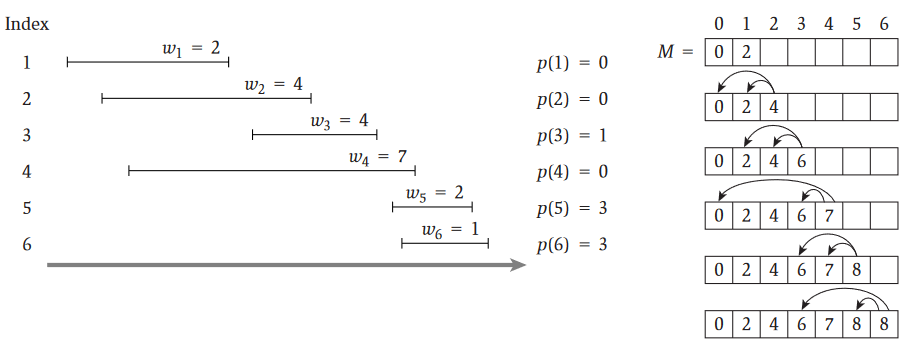
\includegraphics[width = \textwidth]{capitoli/programmazione_dinamica/imgs/iter_comp_opt.png}
      \caption{Figura che mostra le iterazioni per recuperare i valori di OPT}
\end{figure}


Nella sezione precedente, abbiamo sviluppato una soluzione in tempo
polinomiale al problema, progettando: prima un \textbf{algoritmo
      ricorsivo in tempo esponenziale} e poi \textbf{convertendolo (tramite
      memoization) in un algoritmo ricorsivo efficiente} che consultava un
array globale M di soluzioni ottimali per sottoproblemi. Per capire
davvero i concetti della programmazione dinamica, è utile formulare una
versione essenzialmente equivalente dell'algoritmo. \textbf{È questa
      nuova formulazione che cattura in modo più esplicito l'essenza della
      tecnica di programmazione dinamica e servirà come modello generale per
      gli algoritmi che svilupperemo nelle sezioni successive}.

\begin{lstlisting}[language=Python, mathescape=true]
Sort jobs by finish time so that f1 $\le$ f2 $\le$ ... $\le$ fn. 
  Compute p(1), p(2), ..., p(n).
  
  M[0] $\leftarrow$ 0
  for j = 1 TO n
    M[j] $\leftarrow$ max { vj + M[p(j)], M[j - 1] }
\end{lstlisting}

Questo approccio fornisce un secondo algoritmo efficiente per risolvere
il problema dell'Weighted Interval Scheduling. I due approcci
(\textbf{ricorsivo con memoization e iterativo}) hanno chiaramente una
grande quantità di sovrapposizioni concettuali, poiché entrambi crescono
dall'intuizione contenuta nella ricorrenza per \texttt{OPT}. Per il
resto del capitolo, svilupperemo algoritmi di programmazione dinamica
usando il secondo tipo di approccio (costruzione iterativa di
sottoproblemi) perché gli algoritmi sono spesso più semplici da
esprimere in questo modo.

\section{Riepilogo}

\begin{itemize}
      \item
            $OPT[j] = \max_{v_j}+OPT[p_j],OPT[j-1]$
      \item
            Per ogni $j$ scelgo se prenderlo o meno
      \item
            Alcuni sottoproblemi vengono scartati (quelli che si sovrappongono al
            $j$ scelto)
      \item
            Per ogni scelta ho due possibilità: \textbf{TEMPO =} $O(n \log n)$
      \item
            Lo spazio è un vettore di $OPT[j]$: \textbf{SPAZIO =} $O(n)$
      \item
            Per ricostruire la soluzione uso un vettore dove per ogni $j$ ho un
            valore booleano che indica se il job fa parte della soluzione:
            \textbf{SPAZIO\_S =} $O(n)$
\end{itemize}
